\chapter{Experiments and Evaluation}\label{ch:experiments}

This chapter evaluates two design choices: exposing split streams to attribution and changing backward routing through game policies. The split-method and game-based campaigns examine localization, faithfulness, robustness, and numerical or computational cost. We retain their checkpoints, sample exclusions, metric conventions, and selection protocols, comparing scores within each campaign. Model-evaluation scores come from the papers; Pascal VOC uncertainty estimates and comparison statistics are recomputed locally using images as independent sampling units.

\section{Experimental Setup}\label{sec:experimental_setup}\label{sec:quantus_evaluation}

The split campaign evaluates pretrained VGG-16 and ResNet-18 on a custom 50-class ImageNet-S subset at $224\times224$ resolution. The source paper reports 50 validation images (one per class) for layer--formula selection and 566 test images. Its released loader selects locally available image--mask pairs without the game campaign's label-agreement filter; these counts alone cannot recover historical sample membership. Explanations target the predicted class, including for misclassified images; localization uses the annotated object mask. Baselines use Captum, Zennit for $\gamma$-LRP, and separate Grad-CAM++ and LayerCAM implementations. Each method retains localization-selected and Pixel-Flipping-selected configurations (full settings and results: Section~\ref{app:saliency} of the supplement).

The split tables report Pixel Flipping as score-drop AUC (PF$^{\mathrm{drop}}_5$, PF$^{\mathrm{drop}}_{20}$; $\uparrow$), perturbing 112 scalar input features per step, and Maximum Sensitivity with 25 perturbations. The revised game campaign reports remaining-logit AUC (PF$_5$, PF$_{20}$; $\downarrow$), with 1,568 scalar features per step, and sensitivity with 50 perturbations on a common 200-image test subset. Both Pixel-Flipping implementations broadcast spatial attribution over color channels, indexing the flattened $C\times H\times W$ input: $150{,}528$ features for RGB images at this resolution. Quantus measures Selectivity, Attribution Localization and Pointing Game. Both campaigns include VGG-16; their ResNet-18 and ResNet-50 scores are not interchangeable. Table abbreviations are AL (Attribution Localization), PG (Pointing Game), Sel (Selectivity), MaxS (Maximum Sensitivity), AvgS (Average Sensitivity), GCAM (Grad-CAM), GCAM++ (Grad-CAM++), LCAM (LayerCAM), IntGrad (Integrated Gradients), and SmGrad (SmoothGrad); Guided GCAM denotes Guided Grad-CAM. Dark blue shading and bold type mark the best values within each caption's comparison; n/r means unreported in the source paper, and n/a means inapplicable.

\section{Split Methods: VGG-16}\label{sec:results_vgg}

\def\colA{0.10}
\def\colB{0.105}
\def\colSpace{0.0015\linewidth}

\begin{figure}[t]
    \centering

    \begin{minipage}[c]{\colA\linewidth}\centering\scriptsize\textbf{Class}\end{minipage}\hspace{\colSpace}%
    \begin{minipage}[c]{\colB\linewidth}\centering\scriptsize\textbf{Original}\end{minipage}\hspace{\colSpace}%
    \begin{minipage}[c]{\colB\linewidth}\centering\scriptsize\textbf{SplitLRP}\\\scriptsize\textbf{$R^{(10,\text{pos})}$ abs}\end{minipage}\hspace{\colSpace}%
    \begin{minipage}[c]{\colB\linewidth}\centering\scriptsize\textbf{LRP $\gamma$=0.25}\\\scriptsize\textbf{layer 5 abs}\end{minipage}\hspace{\colSpace}%
    \begin{minipage}[c]{\colB\linewidth}\centering\scriptsize\textbf{SplitCAM}\\\scriptsize\textbf{$\alpha=0.4$}\\\scriptsize\textbf{$\delta^{(14,g)}$}\end{minipage}\hspace{\colSpace}%
    \begin{minipage}[c]{\colB\linewidth}\centering\scriptsize\textbf{LayerCAM}\\\scriptsize\textbf{layer 14}\end{minipage}\hspace{\colSpace}%
    \begin{minipage}[c]{\colB\linewidth}\centering\scriptsize\textbf{SplitCAM}\\\scriptsize\textbf{$\alpha=0.3$}\\\scriptsize\textbf{$\delta^{(26,g)}$ abs}\end{minipage}\hspace{\colSpace}%
    \begin{minipage}[c]{\colB\linewidth}\centering\scriptsize\textbf{LayerCAM}\\\scriptsize\textbf{layer 26}\end{minipage}\hspace{\colSpace}%
    \begin{minipage}[c]{\colB\linewidth}\centering\scriptsize\textbf{SplitGrad}\\\scriptsize\textbf{$\alpha=0.3$}\\\scriptsize\textbf{$\delta^{(0,+,g)}$}\end{minipage}

    \vspace{0.25cm}

    \begin{minipage}[c]{\colA\linewidth}
        \centering
        \small goldfinch\\[1pt]
        {\scriptsize (0.9996)}
    \end{minipage}\hspace{\colSpace}%
    \begin{minipage}[c]{\colB\linewidth}
        \centering
        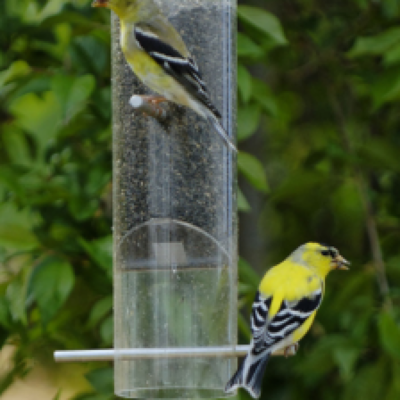
\includegraphics[width=\linewidth]{figures/experiments/saliency_quality/image_0030_ILSVRC2012_val_00030071.JPEG/original_image.png}
    \end{minipage}\hspace{\colSpace}%
    \begin{minipage}[c]{\colB\linewidth}
        \centering
        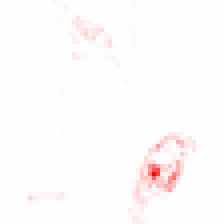
\includegraphics[width=\linewidth]{figures/experiments/saliency_quality/image_0030_ILSVRC2012_val_00030071.JPEG/hybrid_lrp_scaling_max_winnerTakesItAllMaxpool_f10_cam_pp_abs.png}
    \end{minipage}\hspace{\colSpace}%
    \begin{minipage}[c]{\colB\linewidth}
        \centering
        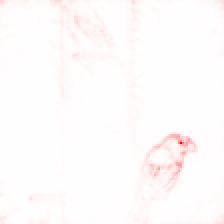
\includegraphics[width=\linewidth]{figures/experiments/saliency_quality/image_0030_ILSVRC2012_val_00030071.JPEG/zennit_lrp_gamma0.25_features_5_abs.png}
    \end{minipage}\hspace{\colSpace}%
    \begin{minipage}[c]{\colB\linewidth}
        \centering
        
\includegraphics[width=\linewidth]{figures/experiments/saliency_quality/image_0030_ILSVRC2012_val_00030071.JPEG/hybrid_cam_shift_40_scale_max_winnerTakesItAllMaxpool_f14_cam_g.png}
    \end{minipage}\hspace{\colSpace}%
    \begin{minipage}[c]{\colB\linewidth}
        \centering
        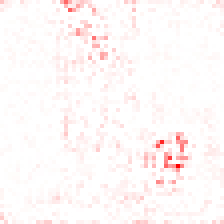
\includegraphics[width=\linewidth]{figures/experiments/saliency_quality/image_0030_ILSVRC2012_val_00030071.JPEG/layer_cam_features_14_relu.png}
    \end{minipage}\hspace{\colSpace}%
    \begin{minipage}[c]{\colB\linewidth}
        \centering
        
\includegraphics[width=\linewidth]{figures/experiments/saliency_quality/image_0030_ILSVRC2012_val_00030071.JPEG/hybrid_cam_shift_30_scale_max_winnerTakesItAllMaxpool_f26_cam_g_abs.png}
    \end{minipage}\hspace{\colSpace}%
    \begin{minipage}[c]{\colB\linewidth}
        \centering
        
\includegraphics[width=\linewidth]{figures/experiments/saliency_quality/image_0030_ILSVRC2012_val_00030071.JPEG/layer_cam_features_26_relu.png}
    \end{minipage}\hspace{\colSpace}%
    \begin{minipage}[c]{\colB\linewidth}
        \centering
        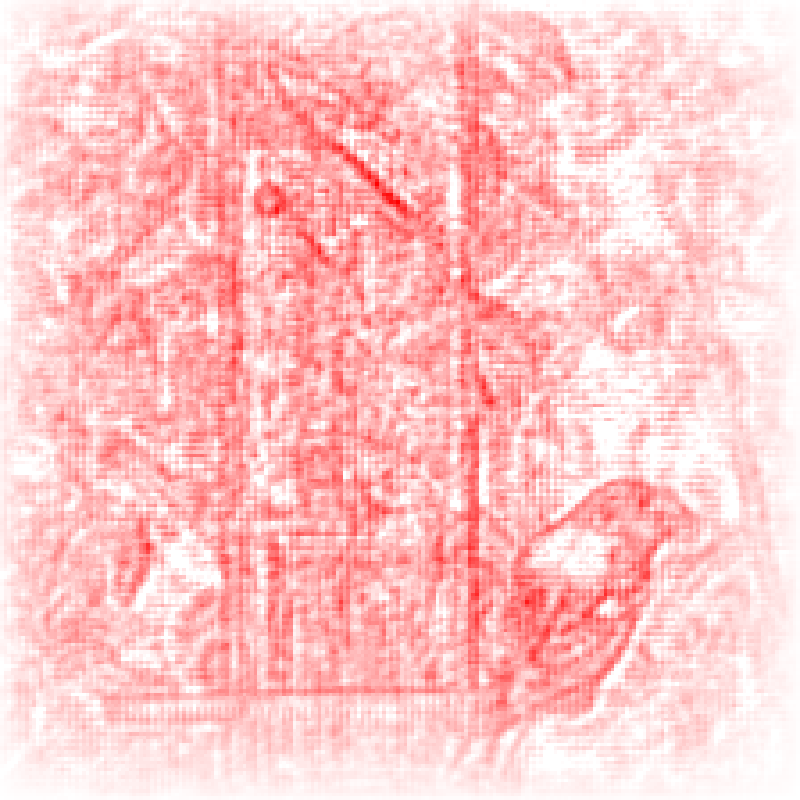
\includegraphics[width=\linewidth]{figures/experiments/saliency_quality/image_0030_ILSVRC2012_val_00030071.JPEG/hybrid_grad_shift_30_max_winnerTakesItAllMaxpool_f0_grad_pp.png}
    \end{minipage}%

    \vspace{0.25cm}

    \begin{minipage}[c]{\colA\linewidth}
        \centering
        \small sulphur butterfly\\[1pt]
        {\scriptsize (0.9999)}
    \end{minipage}\hspace{\colSpace}%
    \begin{minipage}[c]{\colB\linewidth}
        \centering
        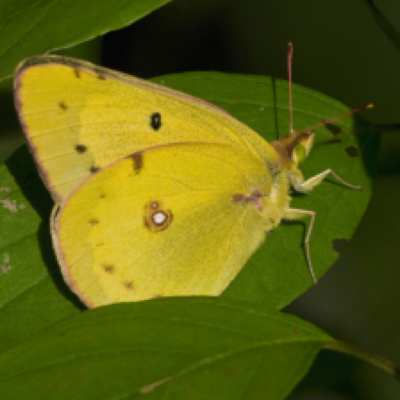
\includegraphics[width=\linewidth]{figures/experiments/saliency_quality/image_0106_ILSVRC2012_val_00019900.JPEG/original_image.png}
    \end{minipage}\hspace{\colSpace}%
    \begin{minipage}[c]{\colB\linewidth}
        \centering
        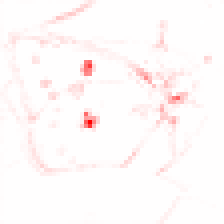
\includegraphics[width=\linewidth]{figures/experiments/saliency_quality/image_0106_ILSVRC2012_val_00019900.JPEG/hybrid_lrp_scaling_max_winnerTakesItAllMaxpool_f10_cam_pp_abs.png}
    \end{minipage}\hspace{\colSpace}%
    \begin{minipage}[c]{\colB\linewidth}
        \centering
        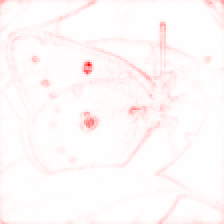
\includegraphics[width=\linewidth]{figures/experiments/saliency_quality/image_0106_ILSVRC2012_val_00019900.JPEG/zennit_lrp_gamma0.25_features_5_abs.png}
    \end{minipage}\hspace{\colSpace}%
    \begin{minipage}[c]{\colB\linewidth}
        \centering
        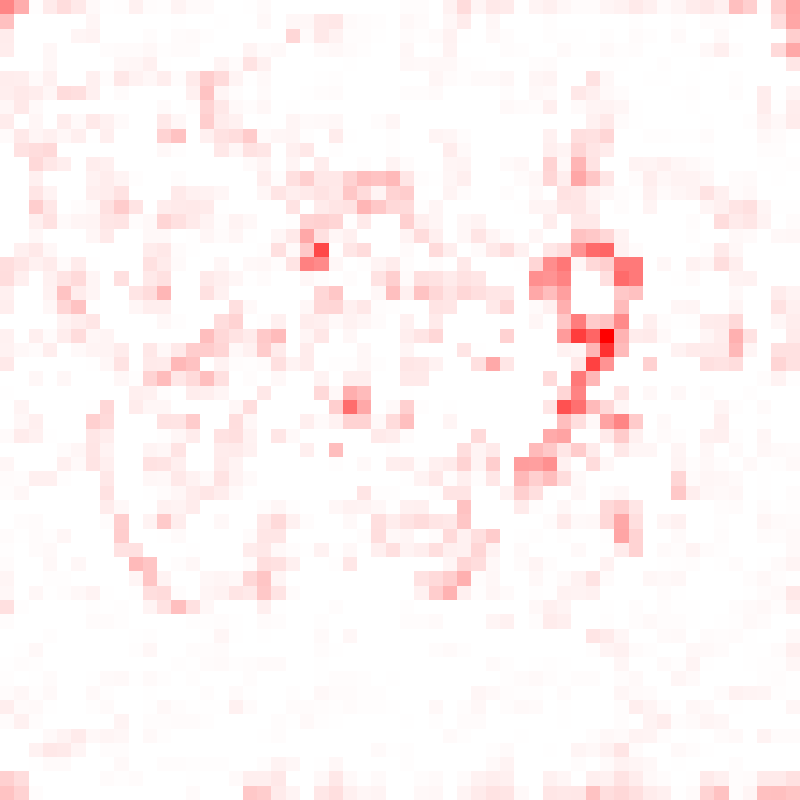
\includegraphics[width=\linewidth]{figures/experiments/saliency_quality/image_0106_ILSVRC2012_val_00019900.JPEG/hybrid_cam_shift_40_scale_max_winnerTakesItAllMaxpool_f14_cam_g.png}
    \end{minipage}\hspace{\colSpace}%
    \begin{minipage}[c]{\colB\linewidth}
        \centering
        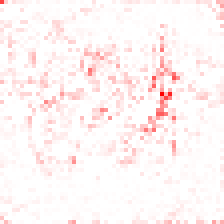
\includegraphics[width=\linewidth]{figures/experiments/saliency_quality/image_0106_ILSVRC2012_val_00019900.JPEG/layer_cam_features_14_relu.png}
    \end{minipage}\hspace{\colSpace}%
    \begin{minipage}[c]{\colB\linewidth}
        \centering
        
\includegraphics[width=\linewidth]{figures/experiments/saliency_quality/image_0106_ILSVRC2012_val_00019900.JPEG/hybrid_cam_shift_30_scale_max_winnerTakesItAllMaxpool_f26_cam_g_abs.png}
    \end{minipage}\hspace{\colSpace}%
    \begin{minipage}[c]{\colB\linewidth}
        \centering
        
\includegraphics[width=\linewidth]{figures/experiments/saliency_quality/image_0106_ILSVRC2012_val_00019900.JPEG/layer_cam_features_26_relu.png}
    \end{minipage}\hspace{\colSpace}%
    \begin{minipage}[c]{\colB\linewidth}
        \centering
        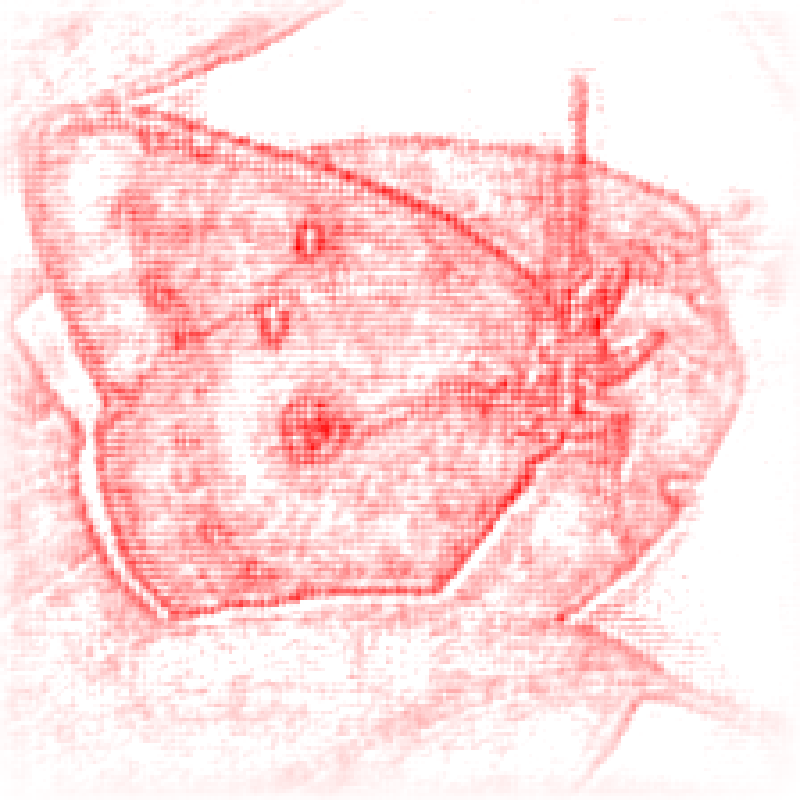
\includegraphics[width=\linewidth]{figures/experiments/saliency_quality/image_0106_ILSVRC2012_val_00019900.JPEG/hybrid_grad_shift_30_max_winnerTakesItAllMaxpool_f0_grad_pp.png}
    \end{minipage}%

    \vspace{0.25cm}

    \begin{minipage}[c]{\colA\linewidth}
        \centering
        \small goldfish\\[1pt]
        {\scriptsize (1.0000)}
    \end{minipage}\hspace{\colSpace}%
    \begin{minipage}[c]{\colB\linewidth}
        \centering
        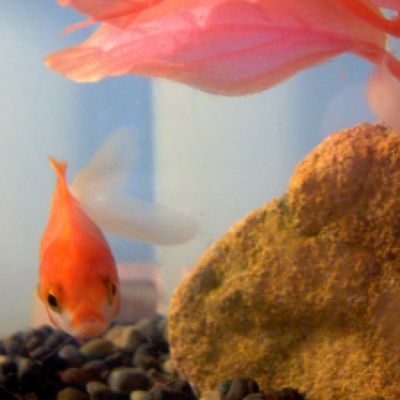
\includegraphics[width=\linewidth]{figures/experiments/saliency_quality/image_0005_ILSVRC2012_val_00020785.JPEG/original_image.png}
    \end{minipage}\hspace{\colSpace}%
    \begin{minipage}[c]{\colB\linewidth}
        \centering
        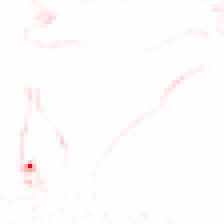
\includegraphics[width=\linewidth]{figures/experiments/saliency_quality/image_0005_ILSVRC2012_val_00020785.JPEG/hybrid_lrp_scaling_max_winnerTakesItAllMaxpool_f10_cam_pp_abs.png}
    \end{minipage}\hspace{\colSpace}%
    \begin{minipage}[c]{\colB\linewidth}
        \centering
        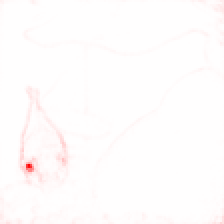
\includegraphics[width=\linewidth]{figures/experiments/saliency_quality/image_0005_ILSVRC2012_val_00020785.JPEG/zennit_lrp_gamma0.25_features_5_abs.png}
    \end{minipage}\hspace{\colSpace}%
    \begin{minipage}[c]{\colB\linewidth}
        \centering
        
\includegraphics[width=\linewidth]{figures/experiments/saliency_quality/image_0005_ILSVRC2012_val_00020785.JPEG/hybrid_cam_shift_40_scale_max_winnerTakesItAllMaxpool_f14_cam_g.png}
    \end{minipage}\hspace{\colSpace}%
    \begin{minipage}[c]{\colB\linewidth}
        \centering
        
\includegraphics[width=\linewidth]{figures/experiments/saliency_quality/image_0005_ILSVRC2012_val_00020785.JPEG/layer_cam_features_14_relu.png}
    \end{minipage}\hspace{\colSpace}%
    \begin{minipage}[c]{\colB\linewidth}
        \centering
        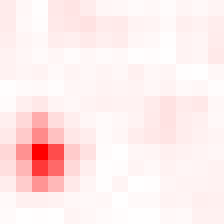
\includegraphics[width=\linewidth]{figures/experiments/saliency_quality/image_0005_ILSVRC2012_val_00020785.JPEG/hybrid_cam_shift_30_scale_max_winnerTakesItAllMaxpool_f26_cam_g_abs.png}
    \end{minipage}\hspace{\colSpace}%
    \begin{minipage}[c]{\colB\linewidth}
        \centering
        
\includegraphics[width=\linewidth]{figures/experiments/saliency_quality/image_0005_ILSVRC2012_val_00020785.JPEG/layer_cam_features_26_relu.png}
    \end{minipage}\hspace{\colSpace}%
    \begin{minipage}[c]{\colB\linewidth}
        \centering
        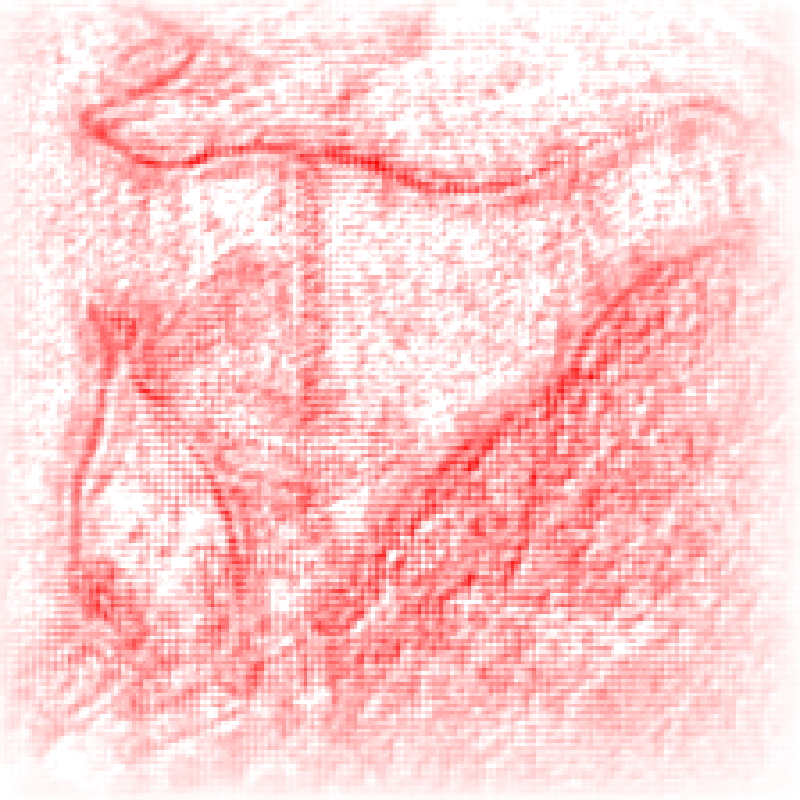
\includegraphics[width=\linewidth]{figures/experiments/saliency_quality/image_0005_ILSVRC2012_val_00020785.JPEG/hybrid_grad_shift_30_max_winnerTakesItAllMaxpool_f0_grad_pp.png}
    \end{minipage}%

    \caption{Saliency map comparison for VGG-16 on our custom ImageNet-S test split. Each row shows the predicted class (with confidence), original image, and saliency maps from different methods.}
    \label{fig:vgg_saliency_comparison_main}
\end{figure}


\paragraph{Qualitative analysis.}
Figure~\ref{fig:vgg_saliency_comparison_main} compares split and baseline saliency maps at their best-performing layers. Mid-layer SplitCAM resembles earlier-layer classical $\gamma$-\ac{lrp}. Against same-layer LayerCAM, it gives more weight across object pixels while emphasizing key features, balancing interpretability and focus (low entropy). For $\alpha \ll 0.5$, SplitGrad yields less focused, finely aligned gradients following image details. We attribute this to Maxout retaining pre-activation information that ReLU discards at inactive neurons. Further examples appear in Section~\ref{app:saliency} of the supplement.

% Source: hiddenMonotonicity (Paper 1), sections/table_main_generated_vgg.tex — numbers verbatim.
\begin{table}[htb!]
    \centering
    \small
    \caption{Comprehensive \ac{xai} evaluation results (VGG-16, ImageNet-S test split). The \emph{wta} abbreviation indicates the use of the ``winner-takes-it-all'' max-pooling implementation; \emph{sc} emphasizes the scaling procedure in the forward pass (Section~\ref{sec:stabilization_dc}). Best values per metric in bold. The bracket notation in the layer column follows the upper indices of the split methods as introduced in Chapter~\ref{ch:saliency}.}
    \label{tab:eval_vgg_main}
    \resizebox{\textwidth}{!}{%
    \begin{tabular}{p{4cm}cc cccccc}
        \toprule
        \textbf{Method} & \textbf{Layer} & \textbf{Abs} & \textbf{Select.} & \textbf{Attr. Loc.} & \textbf{Point.} & \textbf{Pixel Fl. (AUC@5)} & \textbf{Pixel Fl. (AUC@20)} & \textbf{Max Sens.} \\
        & & & \textbf{$\downarrow$} & \textbf{$\uparrow$} & \textbf{$\uparrow$} & \textbf{$\uparrow$} & \textbf{$\uparrow$} & \textbf{$\downarrow$} \\
        \midrule
        \multicolumn{9}{c}{\textit{Split Methods}} \\
        \midrule
        SplitCAM (sc, $\alpha = 0.4$) & (12, g) & n & 4.720 & \textbf{0.651} & 0.912 & 0.213 & 1.794 & 0.389 \\
        SplitCAM (sc, $\alpha = 0.4$) & (14, g) & n & \textbf{2.727} & 0.563 & 0.836 & 0.300 & 2.404 & 1.012 \\
        SplitCAM (sc, $\alpha = 0.4$, wta) & (26, +, g) & y & 4.711 & 0.635 & \textbf{0.938} & 0.165 & 1.590 & 0.456 \\
        SplitGrad ($\alpha = 0.4$, wta) & (12, +, g) & n & 4.735 & 0.635 & 0.883 & 0.186 & 1.756 & 0.651 \\
        SplitGrad ($\alpha = 0.4$, wta) & (14, +, g) & y & 3.287 & 0.540 & 0.818 & 0.249 & 2.186 & 0.857 \\
        SplitLRP (sc, wta) & (26, pos) & y & 5.168 & 0.588 & 0.871 & 0.151 & 1.473 & \textbf{0.282} \\
        \midrule
        \multicolumn{9}{c}{\textit{Baselines (With Layer Optimization)}} \\
        \midrule
        Guided Backprop & 2 & n & 3.276 & 0.632 & 0.883 & 0.281 & 2.302 & 0.571 \\
        Guided Backprop & 5 & n & 3.448 & 0.614 & 0.887 & 0.240 & 2.091 & 0.375 \\
        LayerCAM & 14 & - & 2.792 & 0.576 & 0.798 & \textbf{0.317} & \textbf{2.474} & 2.656 \\
        LayerCAM & 2 & - & 3.128 & 0.580 & 0.855 & 0.300 & 2.191 & 5.508 \\
        LRP $\gamma=0.25$ & 0 & n & 3.189 & 0.615 & 0.680 & 0.218 & 1.918 & 0.519 \\
        LRP $\gamma=0.25$ & 14 & n & 3.593 & 0.577 & 0.611 & 0.279 & 2.255 & 0.491 \\
        \midrule
        \multicolumn{9}{c}{\textit{Baselines}} \\
        \midrule
        DeepLift & 0 & y & 4.447 & 0.551 & 0.726 & 0.281 & 1.945 & 1.053 \\
        Feature Ablation & 0 & y & 6.029 & 0.479 & 0.624 & 0.123 & 1.250 & 0.859 \\
        Gradient SHAP & 0 & y & 4.808 & 0.552 & 0.783 & 0.261 & 1.862 & 1.142 \\
        GradCAM++ & 30 & n & 5.955 & 0.564 & 0.827 & 0.130 & 1.245 & 0.401 \\
        Integrated Gradients & 0 & y & 4.838 & 0.554 & 0.797 & 0.262 & 1.851 & 1.069 \\
        Occlusion & 0 & y & 5.214 & 0.499 & 0.716 & 0.130 & 1.217 & 0.699 \\
        Random Baseline & 0 & y & 3.570 & 0.425 & 0.458 & 0.203 & 1.585 & -- \\
        \bottomrule
    \end{tabular}
    }%
\end{table}


\paragraph{Quantitative analysis.}
Tables~\ref{tab:eval_vgg_main} and~\ref{tab:eval_res_main} compare selected VGG-16 and ResNet-18 configurations on five Quantus metrics: Selectivity, Attribution Localization, Pointing Game accuracy, Pixel Flipping (score-drop AUC, PF$^{\mathrm{drop}}_5$ and PF$^{\mathrm{drop}}_{20}$), and Maximum Sensitivity. \emph{Abs} indicates absolute saliency values before Quantus evaluation. Full results, explanations, layers and parameter configurations appear in Section~\ref{app:saliency} of the supplement.

The backpropagation-based methods depend strongly on layer choice (ablations: Section~\ref{app:ablation} of the supplement).

VGG-16 gains depend on metric and configuration. Table~\ref{tab:eval_vgg_main} gives SplitCAM Pointing Game $0.938$ versus Guided Backprop's $0.887$, Attribution Localization $0.651$ versus Guided Backprop's $0.632$, and Selectivity $2.727$ versus LayerCAM's $2.792$, from different SplitCAM layers. LayerCAM has the highest displayed Pixel Flipping score-drop AUCs, $0.317$ and $2.474$, versus SplitCAM's $0.300$ and $2.404$. SplitLRP has the lowest Maximum Sensitivity, $0.282$, versus Guided Backprop's $0.375$, and higher Pointing Game but lower Attribution Localization and Pixel Flipping scores than the displayed classical $\gamma$-\ac{lrp} configurations.

\section{Split Methods: ResNet-18}\label{sec:results_resnet}

% Source: hiddenMonotonicity (Paper 1), sections/table_main_generated_res.tex — numbers verbatim.
\begin{table}[htb!]
    \centering
    \small
    \caption[Selected interpretability evaluation configurations: ResNet-18]{Selected interpretability evaluation configurations (ResNet-18, ImageNet-S test split). Highlighting identifies the best values among the displayed rows; the full comparison is in Table~\ref{tab:xai_eval_comprehensive_res}. The triples $x.y.z$ are a ResNet-18-internal indexing of the convolutional layer at which the attribution maps are calculated. See the caption of Table~\ref{tab:eval_vgg_main} for further abbreviations and table explanation.}
    \label{tab:eval_res_main}
    \resizebox{\textwidth}{!}{%
    \begin{tabular}{p{4cm}cc cccccc}
        \toprule
    Method & Layer & Abs & Sel$\downarrow$ & AL$\uparrow$ & PG$\uparrow$ & PF$^{\mathrm{drop}}_5$$\uparrow$ & PF$^{\mathrm{drop}}_{20}$$\uparrow$ & MaxS$\downarrow$ \\
         \midrule
        \multicolumn{9}{c}{\textit{SplitCAM Methods}} \\
        \midrule
        SplitCAM (sc, $\alpha = 0.3$, wta) & (1.0.2, g) & n & \cellbest{\textbf{3.503}} & 0.487 & 0.747 & 0.168 & 1.395 & 1.277 \\
        SplitCAM (sc, $\alpha = 0.3$, wta) & (4.1.2, g) & n & 5.654 & \cellbest{\textbf{0.673}} & \cellbest{\textbf{0.972}} & 0.081 & 0.880 & 0.233 \\
        SplitGrad ($\alpha = 0.3$, wta) & (1.0.2, g) & y & 4.449 & 0.513 & 0.777 & 0.149 & 1.266 & 0.813 \\
        SplitGrad ($\alpha = 0.3$, wta) & (4.1.2, g) & y & 5.663 & 0.649 & 0.972 & 0.082 & 0.882 & 0.219 \\
        SplitLRP (sc, wta) & (conv1, pos) & y & 6.313 & 0.506 & 0.587 & 0.056 & 0.697 & 0.755 \\
        \midrule
        \multicolumn{9}{c}{\textit{Baselines (With Layer Optimization)}} \\
        \midrule
        GCAM & 4.1.2 & n & 6.070 & 0.554 & 0.945 & 0.076 & 0.829 & \cellbest{\textbf{0.131}} \\
        LCAM & 2.0.2 & n & 3.690 & 0.549 & 0.865 & 0.144 & 1.428 & 0.913 \\
        LCAM & 4.1.1 & n & 5.661 & 0.664 & 0.971 & 0.083 & 0.890 & 0.227 \\
        LRP $\gamma=0.25$ & conv1 & y & 3.550 & 0.656 & 0.852 & \cellbest{\textbf{0.213}} & 1.737 & 0.521 \\
        \midrule
        \multicolumn{9}{c}{\textit{Baselines}} \\
        \midrule
        Guided Backprop & conv1 & n & 3.517 & 0.621 & 0.867 & 0.212 & \cellbest{\textbf{1.757}} & 0.459 \\
        GradientSHAP & conv1 & y & 5.269 & 0.527 & 0.779 & 0.166 & 1.227 & 1.074 \\
        IntGrad & conv1 & y & 5.265 & 0.528 & 0.777 & 0.167 & 1.226 & 0.994 \\
        Feature Ablation & conv1 & n & 4.655 & 0.136 & 0.684 & 0.188 & 1.388 & 1.077 \\
        Occlusion & conv1 & n & 5.300 & 0.179 & 0.726 & 0.130 & 1.030 & 0.785 \\
        Deconvolution & conv1 & n & 3.934 & 0.484 & 0.666 & 0.147 & 1.203 & 0.751 \\
        Random Baseline & n/a & y & 4.071 & 0.425 & 0.440 & 0.147 & 1.067 & n/r \\
        \bottomrule
    \end{tabular}
    }%
\end{table}


Table~\ref{tab:eval_res_main} reports selected ResNet-18 configurations on the same five metrics, with \emph{Abs} indicating absolute saliency before evaluation (full tables: Section~\ref{app:saliency} of the supplement). SplitCAM has the lowest reported Selectivity, $3.503$, versus $3.517$ for the strongest baseline, Guided Backprop: a difference of $0.014$. SplitCAM and SplitGrad reach Pointing Game $0.972$ versus LayerCAM's $0.971$. Attribution Localization is $0.673$ for SplitCAM and $0.664$ for LayerCAM; Guided Grad-CAM leads the full comparison at $0.742$ (Table~\ref{tab:xai_eval_comprehensive_res}). Baselines retain the best Pixel Flipping and Maximum Sensitivity scores: the gains are metric-specific.

\section{Split-Method Stabilization Ablations}\label{sec:ablations}
\subsection{Backward-Pass Stabilization of the Split Methods}\label{subsec:alpha_ablation}

% Source: hiddenMonotonicity (Paper 1), sections/alpha_ablation_main.tex — numbers verbatim, restyled to booktabs.
\begin{table}[htb]
    \centering
    \footnotesize
    \caption{Comparison of different $\alpha$ parameters with two SplitGrad and SplitCAM base configurations, both in \emph{wta} and \emph{abs} mode, evaluated on the custom ImageNet-S test split.}
    \label{tab:alpha_ablation_main}
    \begin{tabular}{ll cccccc}
    \toprule
    \textbf{Method} & \textbf{Metric} & $\alpha \ .50$ & $\alpha \ .45$ & $\alpha \ .40$ & $\alpha \ .35$ & $\alpha \ .30$ & $\alpha \ .00$ \\
    \midrule
    \multirow{4}{*}{\begin{tabular}[c]{@{}l@{}}\textbf{SplitGrad}\\(26, g)\end{tabular}} & Point. $\uparrow$ & 0.898 & 0.906 & 0.947 & \textbf{0.956} & 0.889 & 0.401 \\
     & Attr. Loc. $\uparrow$ & 0.543 & 0.548 & 0.605 & \textbf{0.617} & 0.535 & 0.449 \\
     & Max Sens. $\downarrow$ & 0.616 & 0.607 & 0.440 & 0.238 & 0.334 & \textbf{0.028} \\
     & Pixel Fl. @20 $\uparrow$ & 1.527 & 1.534 & \textbf{1.581} & 1.448 & 1.317 & 1.247 \\
    \midrule
    \multirow{4}{*}{\begin{tabular}[c]{@{}l@{}}\textbf{SplitCAM}\\(26, +, g)\end{tabular}} & Point. $\uparrow$ & 0.868 & 0.868 & \textbf{0.938} & 0.933 & 0.613 & 0.855 \\
     & Attr. Loc. $\uparrow$ & 0.550 & 0.554 & 0.635 & \textbf{0.663} & 0.403 & 0.513 \\
     & Max Sens. $\downarrow$ & 0.691 & 0.682 & 0.457 & 0.265 & 0.251 & \textbf{0.120} \\
     & Pixel Fl. @20 $\uparrow$ & 1.607 & \textbf{1.609} & 1.585 & 1.499 & 0.853 & 1.507 \\
    \bottomrule
    \end{tabular}
\end{table}


Table~\ref{tab:alpha_ablation_main} varies the shift $\alpha$ for two selected SplitGrad and SplitCAM configurations on the custom ImageNet-S test split. As in Section~\ref{sec:stabilization_dc}, $\alpha = 0$ leaves the backward pass unstabilized; $\alpha = 0.5$ gives local sensitivities resembling scaled original-network gradients. Reducing $\alpha$ from $0.5$ to $0.4$ improves both configurations' Pointing Game and Attribution Localization, while SplitCAM's PF$^{\mathrm{drop}}_{20}$ falls from $1.607$ to $1.585$. SplitGrad peaks in PF$^{\mathrm{drop}}_{20}$ at $\alpha = 0.4$ and localization at $\alpha = 0.35$; SplitCAM's Pointing Game and Attribution Localization peak at $0.4$ and $0.35$, respectively. Both minimize Maximum Sensitivity at $\alpha = 0$. The sweep supports metric-dependent $\alpha$ choices; numerical stabilization and attribution-rule changes remain confounded. Section~\ref{app:ablation} of the supplement (Table~\ref{tab:alpha_comparison_by_method}) gives the full grid and compares convex with winner-takes-it-all max-pooling.

For the same SplitCAM configuration, Tables~\ref{tab:eval_vgg_main} and~\ref{tab:alpha_ablation_main} retain conflicting source values: PF$^{\mathrm{drop}}_{20}=1.590$ versus $1.585$ and MaxS$=0.456$ versus $0.457$. Resolving this discrepancy requires unavailable per-image results.

\paragraph{Forward-pass stabilization.}
Without forward stabilization (Section~\ref{sec:stabilization_dc}), late VGG-16 split activations grow to order $10^{18}$, producing errors of order $10^{9}$; SplitLRP produces nearly uniform maps. Scaling outperforms shifting on every reported metric in the two early-layer SplitLRP configurations. At later layers, shifting gives higher Attribution Localization and Pixel-Flipping score-drop AUC, scaling lowers Maximum Sensitivity, and Pointing Game depends on configuration (supplement Table~\ref{tab:lrp_scale_shift_comparison}; unstabilized and shift-stabilized SplitCAM grids: Tables~\ref{tab:alpha_comparison_none} and~\ref{tab:alpha_comparison_shift}).

\section{Game-Based Case Study}\label{sec:results_vit}\label{sec:saliency_results}\label{ptnb:sec:experiments}\label{ptnb:sec:case-study}



\paragraph{Setup.}
We evaluate \ac{rg} and \ac{sg} against standard backward baselines (Section~\ref{ptnb:app:baselines})
on VGG-16~\parencite{Simonyan2015}, ResNet-50~\parencite{He2016resnet}, and
ViT-B/16~\parencite{Dosovitskiy2021vit}, using PyTorch~\parencite{Paszke2019PyTorch} and torchvision ImageNet-1K
checkpoints~\parencite{Deng2009,Russakovsky2015ilsvrc}\footnote{Checkpoint documentation: \url{https://docs.pytorch.org/vision/stable/models.html}; the weight identifiers used here are listed in Section~\ref{app:extended_protocol}.}, on a 50-class
ImageNet-S subset~\parencite{gao2022luss} at $224{\times}224$ (50-image validation split, 565-image
test split), and on Pascal VOC 2012~\parencite{Everingham2010voc}\footnote{Release documentation: \url{https://www.robots.ox.ac.uk/~vgg/projects/pascal/VOC/voc2012/}.}. For the game campaign, the $752$ released ImageNet-S50 annotation records are filtered to $616$ whose class agrees with the official ILSVRC2012 label; one image per class is selected for validation with seed $42$, and one of the remaining $566$ test images is excluded because its object mask is outside the center crop. The explanation target is the dataset class, including on misclassified images (Section~\ref{ptnb:app:protocol}). ImageNet-S provides the pixel masks
required by the localization metrics; ImageNet boxes over-credit mass anywhere inside the box. All
metrics are computed through Quantus~\parencite{Hedstrom2023} (definitions in
Section~\ref{ptnb:app:metrics}): localization (\ac{ptnbAttrLoc}, \ac{ptnbPG}, Top-$k$ Intersection (TK);
$\uparrow$), faithfulness (Pixel Flipping area under the remaining-logit curve over the first 5\% and 20\% of flips
(PF$_5$, PF$_{20}$), \ac{ptnbSel}; $\downarrow$), robustness (Maximum Sensitivity (MaxS), Average
Sensitivity (AvgS); $\downarrow$). Baselines run in their reference implementations (lxt, zennit,
captum, pytorch-grad-cam, and the authors' code for \acs{ptnbTIBAV} and \acs{ptnbGAE}) at the authors'
settings, plus declared grids~\parencite{Achtibat2024AttnLRP,Anders2021Zennit,kokhlikyan2020captum,Gildenblat2021gradcam,Chefer2021GenericAttention,Chefer2021ICCV}. \ac{rg} analytical modes are
reported alongside each configuration: temperature $\tau$, risk aversion $\lambda$ (softmax-shift
variant $\lambda_{\mathrm{sm}}$ on \ac{vit} attention logits), \ac{lrp} stabilizer $\varepsilon$,
equivariant-Reynolds sample count $N$.

\paragraph{Protocol.}
Methods are evaluated under a two-stage protocol that treats baselines and our games alike. Stage~1
runs a grid search on the validation split (one image per class) for every method with tunable
parameters, including DAVE (Section~\ref{ptnb:app:grids}, Table~\ref{ptnb:tab:main-search-grid}; \nValGrid{}
configurations in total). Stage~2 picks, for each method, the \emph{loc} configuration with the
best localization rank-sum over $\{\text{AL}, \text{PG}, \text{TK}\}$ and, independently, the
\emph{faith} configuration with the best faithfulness rank-sum over $\{\text{PF}_5, \text{PF}_{20},
    \text{Sel}\}$, and evaluates both once on the test split, with 95\% percentile-bootstrap confidence
intervals~\parencite{Efron1993bootstrap} and Holm-corrected~\parencite{Holm1979} paired tests against the
best row of each metric (Section~\ref{ptnb:app:stats}); for \ac{rg} / \ac{rg}+Eq we additionally show
the $\alpha\beta$-\ac{lrp} anchor $(\alpha,\beta,\varepsilon,\tau){=}(2,1,0.5,1)$ as a
theorem-driven reference (Theorem~\ref{ptnb:thm:lrp-recovery}). Localization is a natural target for
modes designed to control routing focus, and object annotations provide external ground truth:
\textcite{Kohlbrenner2020} compare \ac{lrp} rule composites by the share of positive relevance inside
ground-truth bounding boxes; we use absolute attribution mass and pixel masks. The main table reports the loc row of every
method; since mask agreement is not faithfulness, the faith rows of all methods are reported in
Section~\ref{ptnb:app:results}.

\begin{table}[H]
    \centering
    \caption[ViT-B/16 on the ImageNet-S test split]{ViT-B/16 on the ImageNet-S test split ($n{=}565$; MaxS/AvgS on a fixed random subset of
    200 test images). \textbf{Bold}, dark shading: best in column; $^{\approx}$, light shading: not
    significantly different from the best (paired bootstrap / McNemar, Holm-corrected, $p\ge0.05$);
    small numbers: 95\% percentile-bootstrap confidence intervals over test images
    (Section~\ref{ptnb:app:stats}). One row per method, selected on the validation split by the
    localization rank-sum (faithfulness-selected rows and further baselines:
    Section~\ref{ptnb:app:results}); the RG anchor is the exact $\alpha\beta$-\ac{lrp} representation
    (Theorem~\ref{ptnb:thm:lrp-recovery}). $t$/img: seconds per image on one GPU. Config: SmoothGrad
    averages $N$ samples at noise level $\sigma$ relative to the input range; LRP-$\gamma$ has
    stabilizer $\varepsilon$ and positive-weight boost $\gamma$; AttnLRP has layer-type parameters
    $\gamma_{\mathrm{conv}}, \gamma_{\mathrm{lin}}, \varepsilon_{\mathrm{attn}}$; KernelSHAP draws $N$
    samples for $M$ superpixels; \ac{rg} modes as in Table~\ref{ptnb:tab:modes}.\PrelimTag}
    \label{ptnb:tab:eval-vit}\label{tab:eval-vit}
\TableContent{
    \scriptsize
    \resizebox{\textwidth}{!}{\begin{tabular}{@{}l l c c c c c c c c c@{}}
\toprule
Method & Config & AL$\uparrow$ & PG$\uparrow$ & TK$\uparrow$ & PF$_5$$\downarrow$ & PF$_{20}$$\downarrow$ & Sel$\downarrow$ & MaxS$\downarrow$ & AvgS$\downarrow$ & $t$/img \\
\midrule
Gradient & fixed & \begin{tabular}[t]{@{}c@{}}0.411\\[-1pt]{\tiny[0.389,0.432]}\end{tabular} & \begin{tabular}[t]{@{}c@{}}0.361\\[-1pt]{\tiny[0.322,0.402]}\end{tabular} & \begin{tabular}[t]{@{}c@{}}0.386\\[-1pt]{\tiny[0.359,0.413]}\end{tabular} & \begin{tabular}[t]{@{}c@{}}8.45\\[-1pt]{\tiny[8.33,8.56]}\end{tabular} & \begin{tabular}[t]{@{}c@{}}8.08\\[-1pt]{\tiny[7.94,8.22]}\end{tabular} & \begin{tabular}[t]{@{}c@{}}6.033\\[-1pt]{\tiny[5.905,6.154]}\end{tabular} & \begin{tabular}[t]{@{}c@{}}1.290\\[-1pt]{\tiny[1.233,1.351]}\end{tabular} & \begin{tabular}[t]{@{}c@{}}0.922\\[-1pt]{\tiny[0.893,0.953]}\end{tabular} & \textbf{0.02} \\
SmGrad & $N{=}50,\sigma/\mathrm{range}{=}0.2$ & \begin{tabular}[t]{@{}c@{}}0.517\\[-1pt]{\tiny[0.498,0.536]}\end{tabular} & \begin{tabular}[t]{@{}c@{}}0.706\\[-1pt]{\tiny[0.667,0.743]}\end{tabular} & \begin{tabular}[t]{@{}c@{}}0.675\\[-1pt]{\tiny[0.654,0.694]}\end{tabular} & \begin{tabular}[t]{@{}c@{}}8.10\\[-1pt]{\tiny[7.96,8.24]}\end{tabular} & \begin{tabular}[t]{@{}c@{}}7.02\\[-1pt]{\tiny[6.83,7.20]}\end{tabular} & \begin{tabular}[t]{@{}c@{}}5.029\\[-1pt]{\tiny[4.894,5.163]}\end{tabular} & \begin{tabular}[t]{@{}c@{}}0.597\\[-1pt]{\tiny[0.569,0.630]}\end{tabular} & \begin{tabular}[t]{@{}c@{}}0.468\\[-1pt]{\tiny[0.451,0.485]}\end{tabular} & 1.12 \\
\midrule
LRP-$\gamma$ & $\varepsilon{=}0.1,\gamma{=}2$ & \begin{tabular}[t]{@{}c@{}}0.644\\[-1pt]{\tiny[0.628,0.660]}\end{tabular} & \begin{tabular}[t]{@{}c@{}}0.873\\[-1pt]{\tiny[0.844,0.899]}\end{tabular} & \begin{tabular}[t]{@{}c@{}}0.816\\[-1pt]{\tiny[0.800,0.832]}\end{tabular} & \begin{tabular}[t]{@{}c@{}}7.93\\[-1pt]{\tiny[7.78,8.08]}\end{tabular} & \begin{tabular}[t]{@{}c@{}}6.64\\[-1pt]{\tiny[6.44,6.83]}\end{tabular} & \cellbest{\begin{tabular}[t]{@{}c@{}}\textbf{4.451}\\[-1pt]{\tiny[4.324,4.572]}\end{tabular}} & \begin{tabular}[t]{@{}c@{}}0.300\\[-1pt]{\tiny[0.287,0.314]}\end{tabular} & \begin{tabular}[t]{@{}c@{}}0.218\\[-1pt]{\tiny[0.210,0.226]}\end{tabular} & 0.08 \\
AttnLRP & $\gamma_{\mathrm{conv}}{=}0.25,\gamma_{\mathrm{lin}}{=}0.05,\varepsilon_{\mathrm{attn}}{=}0.25$ & \begin{tabular}[t]{@{}c@{}}0.644\\[-1pt]{\tiny[0.628,0.660]}\end{tabular} & \begin{tabular}[t]{@{}c@{}}0.855\\[-1pt]{\tiny[0.825,0.883]}\end{tabular} & \begin{tabular}[t]{@{}c@{}}0.809\\[-1pt]{\tiny[0.794,0.825]}\end{tabular} & \cellbest{\begin{tabular}[t]{@{}c@{}}\textbf{7.77}\\[-1pt]{\tiny[7.61,7.93]}\end{tabular}} & \cellbest{\begin{tabular}[t]{@{}c@{}}\textbf{6.43}\\[-1pt]{\tiny[6.23,6.62]}\end{tabular}} & \begin{tabular}[t]{@{}c@{}}4.582\\[-1pt]{\tiny[4.452,4.706]}\end{tabular} & \begin{tabular}[t]{@{}c@{}}0.456\\[-1pt]{\tiny[0.430,0.484]}\end{tabular} & \begin{tabular}[t]{@{}c@{}}0.342\\[-1pt]{\tiny[0.324,0.364]}\end{tabular} & 0.10 \\
\midrule
TIBAV & fixed & \begin{tabular}[t]{@{}c@{}}0.615\\[-1pt]{\tiny[0.597,0.634]}\end{tabular} & \begin{tabular}[t]{@{}c@{}}0.878\\[-1pt]{\tiny[0.851,0.904]}\end{tabular} & \begin{tabular}[t]{@{}c@{}}0.782\\[-1pt]{\tiny[0.759,0.805]}\end{tabular} & \begin{tabular}[t]{@{}c@{}}8.13\\[-1pt]{\tiny[8.01,8.24]}\end{tabular} & \begin{tabular}[t]{@{}c@{}}7.60\\[-1pt]{\tiny[7.46,7.74]}\end{tabular} & \begin{tabular}[t]{@{}c@{}}4.906\\[-1pt]{\tiny[4.774,5.033]}\end{tabular} & \begin{tabular}[t]{@{}c@{}}1.062\\[-1pt]{\tiny[1.001,1.126]}\end{tabular} & \begin{tabular}[t]{@{}c@{}}0.512\\[-1pt]{\tiny[0.486,0.540]}\end{tabular} & 0.15 \\
GAE & fixed & \begin{tabular}[t]{@{}c@{}}0.533\\[-1pt]{\tiny[0.514,0.551]}\end{tabular} & \begin{tabular}[t]{@{}c@{}}0.743\\[-1pt]{\tiny[0.708,0.779]}\end{tabular} & \begin{tabular}[t]{@{}c@{}}0.649\\[-1pt]{\tiny[0.623,0.677]}\end{tabular} & \begin{tabular}[t]{@{}c@{}}8.13\\[-1pt]{\tiny[8.01,8.25]}\end{tabular} & \begin{tabular}[t]{@{}c@{}}7.62\\[-1pt]{\tiny[7.47,7.76]}\end{tabular} & \begin{tabular}[t]{@{}c@{}}5.098\\[-1pt]{\tiny[4.961,5.231]}\end{tabular} & \begin{tabular}[t]{@{}c@{}}0.525\\[-1pt]{\tiny[0.494,0.558]}\end{tabular} & \begin{tabular}[t]{@{}c@{}}0.368\\[-1pt]{\tiny[0.346,0.391]}\end{tabular} & 0.03 \\
\midrule
KernelSHAP & $N{=}2M{+}2048$, 80 superpixels & \begin{tabular}[t]{@{}c@{}}0.565\\[-1pt]{\tiny[0.548,0.583]}\end{tabular} & \cellbest{\begin{tabular}[t]{@{}c@{}}\textbf{0.961}\\[-1pt]{\tiny[0.945,0.977]}\end{tabular}} & \cellapprox{\begin{tabular}[t]{@{}c@{}}0.823\textsuperscript{$\approx$}\\[-1pt]{\tiny[0.799,0.848]}\end{tabular}} & \begin{tabular}[t]{@{}c@{}}8.29\\[-1pt]{\tiny[8.18,8.40]}\end{tabular} & \begin{tabular}[t]{@{}c@{}}7.50\\[-1pt]{\tiny[7.35,7.65]}\end{tabular} & \begin{tabular}[t]{@{}c@{}}5.140\\[-1pt]{\tiny[5.012,5.261]}\end{tabular} & \begin{tabular}[t]{@{}c@{}}0.897\\[-1pt]{\tiny[0.868,0.928]}\end{tabular} & \begin{tabular}[t]{@{}c@{}}0.650\\[-1pt]{\tiny[0.632,0.667]}\end{tabular} & 6.71 \\
\midrule
RG anchor & $\tau{=}1$ & \begin{tabular}[t]{@{}c@{}}0.509\\[-1pt]{\tiny[0.490,0.528]}\end{tabular} & \begin{tabular}[t]{@{}c@{}}0.724\\[-1pt]{\tiny[0.685,0.759]}\end{tabular} & \begin{tabular}[t]{@{}c@{}}0.699\\[-1pt]{\tiny[0.678,0.720]}\end{tabular} & \begin{tabular}[t]{@{}c@{}}8.19\\[-1pt]{\tiny[8.05,8.31]}\end{tabular} & \begin{tabular}[t]{@{}c@{}}6.97\\[-1pt]{\tiny[6.78,7.15]}\end{tabular} & \begin{tabular}[t]{@{}c@{}}4.854\\[-1pt]{\tiny[4.732,4.972]}\end{tabular} & \cellbest{\begin{tabular}[t]{@{}c@{}}\textbf{0.166}\\[-1pt]{\tiny[0.161,0.172]}\end{tabular}} & \begin{tabular}[t]{@{}c@{}}0.120\\[-1pt]{\tiny[0.117,0.124]}\end{tabular} & 0.10 \\
RG & $\tau{=}0.4,\lambda_{\mathrm{sm}}{=}{-}10,\sigma^2{=}5,\varepsilon{=}0.1$ & \cellbest{\begin{tabular}[t]{@{}c@{}}\textbf{0.711}\\[-1pt]{\tiny[0.692,0.730]}\end{tabular}} & \begin{tabular}[t]{@{}c@{}}0.825\\[-1pt]{\tiny[0.793,0.855]}\end{tabular} & \begin{tabular}[t]{@{}c@{}}0.788\\[-1pt]{\tiny[0.768,0.808]}\end{tabular} & \begin{tabular}[t]{@{}c@{}}8.27\\[-1pt]{\tiny[8.14,8.39]}\end{tabular} & \begin{tabular}[t]{@{}c@{}}7.48\\[-1pt]{\tiny[7.31,7.64]}\end{tabular} & \begin{tabular}[t]{@{}c@{}}5.109\\[-1pt]{\tiny[4.987,5.226]}\end{tabular} & \begin{tabular}[t]{@{}c@{}}0.729\\[-1pt]{\tiny[0.685,0.777]}\end{tabular} & \begin{tabular}[t]{@{}c@{}}0.494\\[-1pt]{\tiny[0.471,0.518]}\end{tabular} & 0.17 \\
RG+Eq anchor & $\tau{=}1,N{=}50$ & \begin{tabular}[t]{@{}c@{}}0.520\\[-1pt]{\tiny[0.501,0.539]}\end{tabular} & \begin{tabular}[t]{@{}c@{}}0.761\\[-1pt]{\tiny[0.726,0.796]}\end{tabular} & \begin{tabular}[t]{@{}c@{}}0.752\\[-1pt]{\tiny[0.729,0.775]}\end{tabular} & \begin{tabular}[t]{@{}c@{}}8.41\\[-1pt]{\tiny[8.29,8.52]}\end{tabular} & \begin{tabular}[t]{@{}c@{}}7.72\\[-1pt]{\tiny[7.56,7.87]}\end{tabular} & \begin{tabular}[t]{@{}c@{}}4.864\\[-1pt]{\tiny[4.742,4.981]}\end{tabular} & \cellapprox{\begin{tabular}[t]{@{}c@{}}0.170\textsuperscript{$\approx$}\\[-1pt]{\tiny[0.165,0.175]}\end{tabular}} & \cellbest{\begin{tabular}[t]{@{}c@{}}\textbf{0.115}\\[-1pt]{\tiny[0.112,0.118]}\end{tabular}} & 4.93 \\
RG+Eq & $\tau{=}0.5,\lambda_{\mathrm{sm}}{=}{-}10,\sigma^2{=}2,N{=}50$ & \begin{tabular}[t]{@{}c@{}}0.698\\[-1pt]{\tiny[0.680,0.717]}\end{tabular} & \begin{tabular}[t]{@{}c@{}}0.855\\[-1pt]{\tiny[0.827,0.883]}\end{tabular} & \cellbest{\begin{tabular}[t]{@{}c@{}}\textbf{0.836}\\[-1pt]{\tiny[0.815,0.857]}\end{tabular}} & \begin{tabular}[t]{@{}c@{}}8.39\\[-1pt]{\tiny[8.28,8.50]}\end{tabular} & \begin{tabular}[t]{@{}c@{}}7.80\\[-1pt]{\tiny[7.65,7.94]}\end{tabular} & \begin{tabular}[t]{@{}c@{}}5.010\\[-1pt]{\tiny[4.889,5.127]}\end{tabular} & \begin{tabular}[t]{@{}c@{}}0.441\\[-1pt]{\tiny[0.421,0.463]}\end{tabular} & \begin{tabular}[t]{@{}c@{}}0.301\\[-1pt]{\tiny[0.290,0.313]}\end{tabular} & 8.66 \\
\bottomrule
\end{tabular}
}
}%
\end{table}

\paragraph{ViT-B/16 (Table~\ref{ptnb:tab:eval-vit}).}
Under the localization-selected protocol, the \ac{rg} family beats every baseline on attribution
localization, including the prior transformer-specific backward methods
AttnLRP~\parencite{Achtibat2024AttnLRP}, our DAVE implementation~\parencite{Wrobel2024} (Section~\ref{ptnb:app:baselines}),
\ac{ptnbTIBAV}~\parencite{Chefer2021GenericAttention} and \ac{ptnbGAE}~\parencite{Chefer2021ICCV}: the selected mode
reaches AL \vitRGlocAL{} against \vitBestBaseAL{} for the best baseline (\vitBestBaseALname), and
\ac{rg}+Eq \vitRGEqlocAL{}, both significantly ahead of every baseline row after Holm correction.
\ac{rg}+Eq also has the highest observed TK (\vitRGEqlocTK{}), but the Holm-corrected tests do not detect a difference from \vitBestBaseTKname{}
at \vitBestBaseTK{} or LRP-$\gamma$ at $0.816$. The pointing game is led by \vitBestBasePGname{} (\vitBestBasePG{}), whose
maps are constant on superpixels: a hit needs only one pixel of the maximal region inside the mask.
Scoring a single pixel drawn from that region instead, KernelSHAP falls below \ac{rg}+Eq, which is
then not significantly below the best baseline (LRP-$\gamma$; Section~\ref{ptnb:app:pg-granularity}).
Among the localization-selected rows, faithfulness favors the \ac{lrp} rules: AttnLRP is best on PF$_5$ and PF$_{20}$ and LRP-$\gamma$ on
Sel (PF$_{20}$ \vitBestBasePFtwenty{} versus \vitRGlocPFtwenty{} for \ac{rg}), and the
faithfulness-selected \ac{rg} row narrows but does not close the gap (PF$_{20}$
\vitRGfaithPFtwenty{}). Across both selection objectives, faithfulness-selected AttnLRP has the lowest PF$_5$, PF$_{20}$ and Selectivity, at $7.64$, $6.12$ and $4.441$, respectively. The two anchors are the most robust rows (MaxS \vitRGanchorMaxS{} and
\vitRGEqanchorMaxS{} versus \vitBestBaseMaxS{} for \vitBestBaseMaxSname{}), whereas the
localization-selected mode reaches MaxS \vitRGlocMaxS{}: sharper routing trades robustness and
faithfulness for localization. \ac{ptnbADF} adds modest overhead (\ac{rg}: \vitRGlocTime\,s vs.\
\vitRGanchorTime\,s base), still below sampling baselines like SmoothGrad or IntGrad; Reynolds
averaging is the only expensive variant (\vitRGEqTime\,s), exceeding even the perturbation method
KernelSHAP (\vitSHAPTime\,s).

\paragraph{Higher $\tau$ spreads attribution into context.}
Localization-optimal modes concentrate mass on the few patches aligning with the mask. Increasing $\tau$ spreads equilibrium routing over more predecessors: the displayed examples retain object focus while extending attribution into context, without establishing which contextual features the model uses. Around the selected ViT-B/16 setting, AL decreases monotonically from $0.723$ at $\tau{=}0.3$ to $0.461$ at $\tau{=}1$; faithfulness is non-monotonic. High $\tau$ shows how localization scores favor concentrated maps within the same game. User-perceived informativeness remains untested.

\paragraph{Cross-dataset transfer (Pascal VOC).}
A natural worry with validation-tuned modes is that the chosen $\tau$, $\lambda_{\mathrm{sm}}$ and
$\sigma^2$ are overfitted to the ImageNet-S 50-class subset. We test transfer on a per-image
disjoint split of Pascal VOC 2012 trainval ($2{,}743$ test (image, foreground-class) samples with
pixel-accurate segmentation masks): \ac{rg} and \ac{rg}+Eq use the \emph{same} mode parameters as
Table~\ref{ptnb:tab:eval-vit} without any VOC-side re-tuning, while every baseline gets a fresh
per-method validation grid on the new pool. This tests the portability of the selected parameters
across these datasets for the same pretrained model, without identifying whether the underlying
structure is model-specific or dataset-specific. The localization lead carries over (AL
\vocRGlocAL{} for \ac{rg} and \vocRGEqlocAL{} for \ac{rg}+Eq versus \vocBestBaseAL{} for
\vocBestBaseALname{}, both significant against every baseline row), while TK and PG are led by
\ac{ptnbTIBAV} and the perturbation methods, and faithfulness by the \ac{lrp} rules
(Section~\ref{ptnb:app:voc-cross-data}).

\paragraph{VGG-16 and ResNet-50 (Section~\ref{ptnb:app:results}).}
On CNNs, where \ac{lrp}-type rules are strong, localization-selected \ac{rg} leads AL within that selection: clearly on VGG-16 (\vggRGlocAL{} versus \vggBestBaseAL{} for \vggBestBaseALname{}) and narrowly on ResNet-50 (\resRGlocAL{} versus \resBestBaseAL{} for \resBestBaseALname{}). The ResNet-50 difference is not Holm-significant (adjusted $p=0.420$), so its numerical lead does not establish superiority. Across both objectives, VGG-16's strongest baseline AL is faithfulness-selected LRP-$\varepsilon$ at $0.639$, below \ac{rg}'s \vggRGlocAL{}. Pixel Flipping favors LRP-$\varepsilon$ for VGG-16 PF$_5$ ($12.43$), LRP-$\gamma$ for VGG-16 PF$_{20}$ ($7.89$ versus LRP-$\varepsilon$'s $8.17$), and LRP-$\gamma$ for both ResNet-50 metrics; \ac{cam} and perturbation methods lead TK and PG. VGG-16's risk-averse \ac{sg} is most robust (MaxS \vggSGlocMaxS{} versus \vggBestBaseMaxS{} for \vggBestBaseMaxSname{}).

\subsection{Game-Method Ablations}\label{subsec:mode_ablation}

Section~\ref{ptnb:app:abl-one-factor} varies one mode around each validation-selected configuration on 565 test images; these diagnostics do not affect selection. Section~\ref{ptnb:app:pg-granularity} controls Pointing Game for map granularity, and Section~\ref{ptnb:app:abl-gradient-fallback} compares composite Value-routing attention with a gradient fallback. The analyses reveal trade-offs among mask agreement, perturbation faithfulness and robustness.
